\documentclass{article}
% Language setting
% Replace `english' with e.g. `spanish' to change the document language
\usepackage[english,russian]{babel}
\usepackage{amsmath}

%графика
\usepackage{wrapfig}
\usepackage{graphicx}
\usepackage{pgfplots}
\usepackage{tikz}


\usepackage{tcolorbox}

% Set page size and margins
% Replace `letterpaper' with `a4paper' for UK/EU standard size
\usepackage[letterpaper,top=2cm,bottom=2cm,left=3cm,right=3cm,marginparwidth=1.75cm]{geometry}

% Useful packages
\usepackage{amsmath}
\usepackage{amssymb}
\usepackage{graphicx}
\usepackage{fixltx2e}
\usepackage[colorlinks=true, allcolors=blue]{hyperref}

\usepackage{geometry}
\geometry{left=25mm,right=25mm,
 top=25mm,bottom=25mm}

\title{Количественная аналитика.\\
Лекции. Недели 1-2. \\
Derivatives pricing. Греки и введение  в деривативы.}
\author{Алпатов Иван}

% Колонтитулы
\usepackage{fancyhdr}
\pagestyle{fancy}
\renewcommand{\headrulewidth}{0.1mm}  
\renewcommand{\footrulewidth}{0.1mm}
\lfoot{}
\rfoot{\thepage}
\cfoot{}
\rhead{CMF-2022}
\chead{}

\begin{document}
\maketitle

% Оглавление
\setcounter{tocdepth}{1} % {2} - в оглавлении участвуют chapter, section и subsection. {1} - только chapter и section
\renewcommand\contentsname{Contents}
\tableofcontents
\newpage

% \section{Dictionary, Definitions, Abbreviations}

% \subsection{Dictionary}
% \begin{itemize}
%     \item IR - Interest rate - процентная ставка.
%     \item Compounding - платежи (idk)
% \end{itemize}

% \subsection{Definitions and Abbreviations}
% \begin{itemize}
%     \item SAR - Stated annual rate.
%     \item EAR - Effective annual rate.
%     \item FoC - Frequency of Compounding
%     \item PMT - Payment
%     \item r - Interest rate (at the moment). 
% \end{itemize}

\renewcommand{\labelitemi}{\tiny$\bullet$}
\renewcommand{\figurename}{Рис.}

 \section{Немного про биномиальную модель}
 Здесь и далее BSM - Black Scholes (Merton) model (модель Блека-Шоулза-Мертона), PDE - partial differential equation (уравнение в частных производных).
 
\textbf{Биномиальная модель} - годится, в основном, только для обучения. На практике почти не используется. На ней освоили понятие реплицирущего портфеля. Такой портфель состоит из некоторого количества underlying (базового) актива, так, чтобы было безразлично, куда идёт цена (безрисковый портфель). При увеличении количества шагов до бесконечности биномиальная модель сходится к BSM (при стремлении \(N \rightarrow \infty\) в силу центральной предельной теоремы биномиальное распределение стремится к нормальному)

\section{Использование BSM}
\begin{itemize}
     \item Если используем BSM, то для того, чтобы вычислить цену даже ванильного опциона, нужно знать довольно много параметров: волатильность \(\sigma\), maturity \(T\) - время экспирации, strike price (цена страйк) \(K\), безрисковая процентная ставка (risk-free rate)  \(r\), тип оциона - call или put. 
     
    \item Процентная ставка \(r\) - та, что доступна для какого-то института (то есть та, по которой можем занимать и класть деньги, потому что именно это используется в выводе формулы BSM). Например, межбанковская. 
    
    \item Как считать волатильность \(\sigma\)? Считаем историческую (как показывалось на предыдущей лекции по BSM). Переходим к логарифмическим доходностям, считаем несмещенную дисперсию и корень из нее и есть волатильность. 
    
    \[x_t = \ln{\frac{P_t}{P_{t-1}}}\]
    \[\sigma_x = \sqrt{\frac{1}{N-1} \sum_{i=1}^n (x_t - \bar x)^2}\]
    
    Также, важно, что для BSM нам нужно значение годовой волатильности, поэтому если считаем по дням, неделям, месяцам, нужно домножить на корень из количества периодов в году (формула была на предыдущей лекции по BSM)
    \[\sigma_{annually} = \sqrt{52}\sigma_{weekly}, \, \sigma_{annually} \approx \sqrt{252}\sigma_{weekly}\]
    
    \item Встаёт вопрос, по каким периодам лучше считать волатильность. Пример: пусть посчитанная по дням волатильность составила \(\sigma_{daily} = 23\%\), по неделям - \(\sigma_{weekly} = 27\%\) (оба значения - годовая волатильность). Это означает, что было нарушено условие того, что underlying актив является геометрическим броуновским движением, поскольку если бы это было так, то доходности были бы распределены нормально, и работала бы формула с домножением на \(\sqrt{T}\). Если это нарушается, то волатильность, посчитанная по дням, не будет соответствовать недельной. 
    
    Как на самом деле правильно считать волатильность - непонятно. Много разных моделей, все, в основном, считают историческую.

 \end{itemize}



\section{Греки}

Есть формула BSM:
\[\frac{\partial V}{\partial t} + r S \frac{\partial V}{\partial S} + \frac{1}{2}\frac{\partial^2 V}{\partial S^2}\sigma^2 S^2 = rV\]

Греки - помогают трейдерам понимать рискованность их позиции, и то, как она будет реагировать на разные изменения на рынке.

\begin{itemize}

    \item \(\theta = \frac{\partial V}{\partial t}\), Тета - частная производная стоимости опциона по времени, "time decay term". Для ванильного опциона \(<0\), так как всё меньше времени для того, чтобы получить выгоду. Уменьшение времени до погашения означает, что вероятность оказаться «в деньгах» для опциона уменьшается.
    
    \item \(\Delta = \frac{\partial V}{\partial S}\), Дельта - изменение цены опциона с изменением цены underlying актива, hedge ratio. 
    
    \item \(\Gamma = \frac{\partial^2 V}{\partial S^2}\), Гамма - выпуклость, производная дельты по цене underlying актива. 
\end{itemize}

Перепишем уравнение BSM с помощью греков:
\[\theta +  \frac{1}{2}\Gamma\sigma^2 S^2 = r(V-\Delta S)\]

Справа - портфель, из вывода BSM, состоящий из одного дериватива в лонг и underlying актива в количестве дельта в шорт. Знаем, что такой портфель должен зарабатывать risk-free rate. Из уравнения видно, что заработок такого портфеля состоит из теты (уменьшает стоимость с течением времени) и гаммы. Gain, который получаем от гаммы, частично компенсируется убытком от теты (time-decay), то есть от того, что осталось меньше времени до экспирации. 

\textbf{Дополнительные греки}, для изучения того, как зависит решение уравнения BSM от параметров:

\begin{itemize}

    \item \(\nu = \frac{\partial V}{\partial \sigma}\), Vega (Вега) - частная производная стоимости опциона по волатильности. Вега положительная для ванильного опциона, потому что чем выше волатильность, тем выше возможность заработка, при этом снизу заработок ограничен. Upside - большой, downside - маленький. 
    
    \item \(Vanna = \frac{\partial^2 V}{\partial S \partial \sigma}\), Ванна - производная дельты по волатильности. 
    
    \item \(Volga = \frac{\partial^2 V}{\partial \sigma^2}\), Волга - вторая производная стоимости опциона по волатильности. 
    
     \item \(\rho = \frac{\partial V}{\partial r}\), Rho (Ро) - производная стоимости опциона по ставке. 
\end{itemize}


Формула BSM - является PDE. Решается с помощью соответствующих формул и численных методов для уравнения теплопроводности. Но есть другой способ находить цену опциона - через т. Гирсанова и мартингальную меру. Цена опциона будет просто матожиданием. 


\section{Вероятностный подход к нахождению цены опциона}

\begin{itemize}
    \item \textbf{Дефлятор} \(D(t)\) - положительный процесс Ито. Нормализуем наш underlying актив на дефлятор.
\[S^D (t) = \frac{S(t)}{D(t)}\]

    \item Мера \(Q^D\) - \textbf{эквивалентная мартингальная мера (риск-нейтральная), порожденная дефлятором} \(D\), если \(S^D (t)\) - \(Q^D\)-мартингал. 

    \item \underline{\textbf{Первая фундаментальная теорема теории прайсинга}}. Если существует дефлятор, такой, что нормализованная цена актива представляет собой мартингал (т.е. существует мартингальная мера), то на рынке отсутствует арбитраж. 

    \item Если условие теоремы выполняется, то нормализованная цена опциона также будет мартингалом (пользуемся тем, что опцион можно реплицировать портфелем из того, что есть на рынке, что в свою очередь при нормализации будет мартингалом) и нормализованная цена в момент времени \(t=0\) будет равна матожиданию нормализованной цены опциона в момент времени \(T\), посчитанному в мартингальной мере. Цена опциона в момент \(T\) равна payoff (функции выплат). Чтобы узнать цену опциона в момент времени \(t=0\) нужно просто нормализованную цену умножить на \(D(0)\).
\end{itemize}

\section{Методы нахождения цены опциона}

\begin{figure}[h]
    \centering 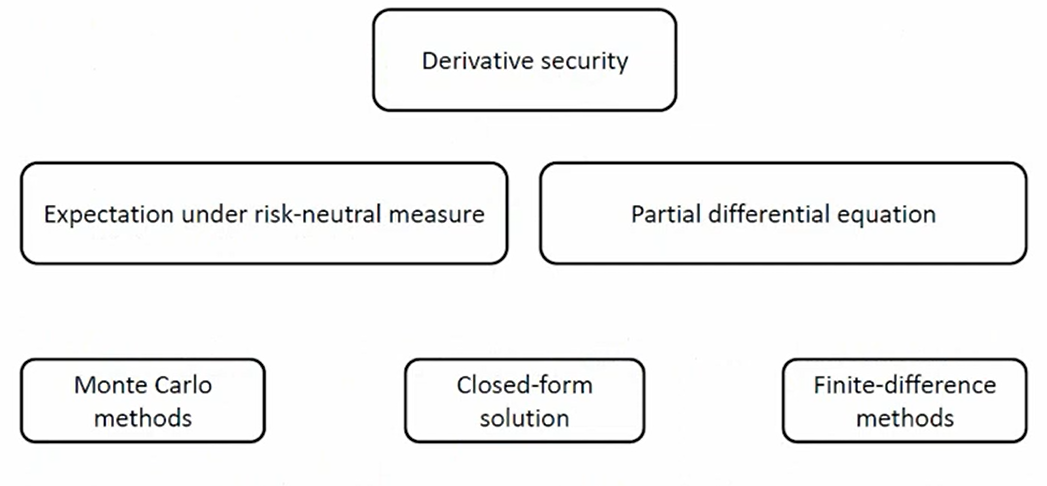
\includegraphics[width=0.9\textwidth]{scheme.png}
\end{figure}
\begin{figure}[h!]
    \centering 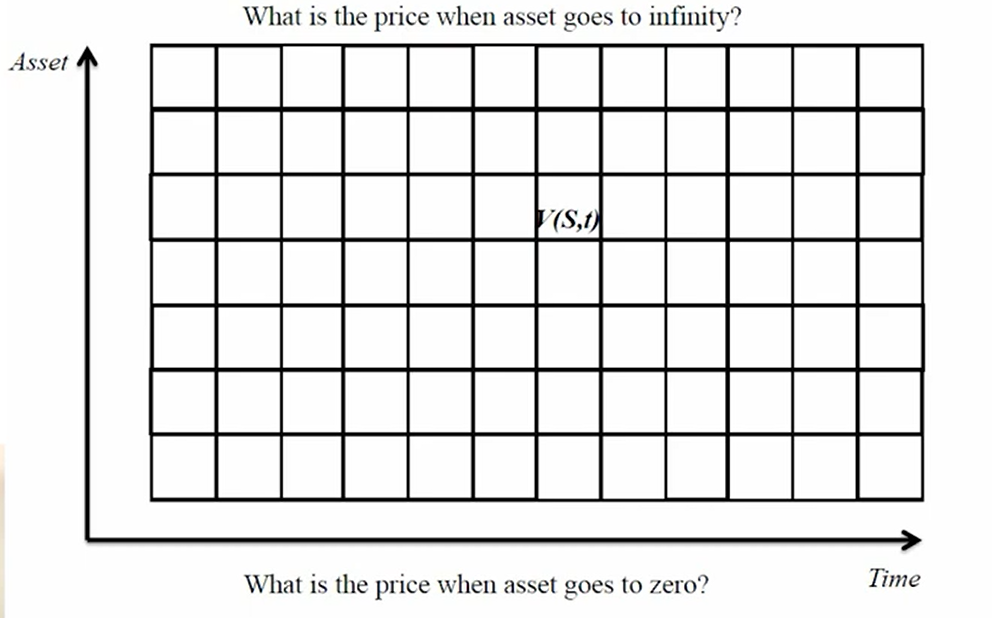
\includegraphics[width=0.8\textwidth]{net.png}
    \caption{Конечно-разностная сетка}
\end{figure}

Есть сложный дериватив. Два глобальных подхода оценить дериватив: через PDE Блека-Шоулза и через риск-нейтральную (мартингальную) меру. Лемма Фейнмана-Каца утверждает, что оба подхода дадут одинаковый результат. Для PDE граничные условия, в основном, будут сложнее, чем для обычного опциона. 

Как можно решить PDE? 
\begin{itemize}
    \item Closed form solution - готовое решение уравнения, формула (как, например, для ванильного опциона). Для большинства деривативов таких решений нет.
    
    \item Численные методы, в основном, конечно-разностные методы решения PDE. Используются конечно-разностные операторы, такие, как: 
    \[\Delta = \delta_{x} V(t, x_j) = \frac{V(t, x_{j+1}) - V(t, x_{j-1})}{2\Delta x}\]
    \[\Gamma = \delta_{xx} V(t, x_j) = \frac{V(t, x_{j+1}) - 2V(t, x_{j}) + V(t, x_{j-1})}{(\Delta x)^2}\]
    \[\theta =  \frac{\partial V}{\partial t} \approx \frac{V(t_{i+1}) - V(t_i)}{\Delta t}\]

\end{itemize}

В подходе с риск-нейтральной мерой обычно применяют методы Монте-Карло. Симулируют большое количество путей, считают по всем выплаты, усредняют, получают ответ. Матожидание считаем численно:
\[V(t) = D(t) E_t^Q (V(T)/D(T))\]

\section{Примеры опционов}

\begin{enumerate}
  \item \textbf{Американский непрерывный барьерный (barrier) опцион}. 
  \begin{itemize}
  \item Зависит от пути, т.е. от движения цены. Например, дает право купить акции по 90, но если цена стала больше 120, то  это право у нас исчезает. Поэтому такой опцион стоит дешевле. Поскольку American option, можно исполнить (exercise) в любой момент. 
  \item Подходит клиентам, которые считают, что знают достаточно точно, в каких границах будет меняться цена. 
  \item Типы (примеры для call option со strike = 90): 
      \begin{itemize}
      \item \textbf{Up-and-out} - право купить по 90, но если когда-нибудь в течение времени действия цена становится выше какого-нибудь барьера (например 120) право пропадает, 
      \item \textbf{Down-and-out} - то же самое, только если цена становится ниже определенного барьера, 
      \item \textbf{Up-and-in} - право появляется, если цена становится выше барьера, 
      \item  \textbf{Down-and-in} - то же самое, только если цена становится ниже барьера.  
      \end{itemize}
        \item Как я понял, прайсится с помощью конечно-разностных методов.
  \end{itemize}
  \item \textbf{Asian basket option (азиатский опцион на корзину)}. Payoff \(g(T)\) определяется по формуле. Сравниваем среднее от взвешенной суммы активов по времени со страйком \(K\).
  
  \[g(T) = (\frac{1}{m} \sum_{i=1}^m B(t_i) - K)^{+}\]
  \[B(t) = \sum_{k=1}^p S_k(t)\]
  
  \(B(t)\) - взвешенная корзина. Т.е. берём несколько акций, каждую со своим весом. Считаем, что \(S_k\) - все являются ГБД (геометрическое броуновское движение). Но, волатильности разные, а также приращения одного винеровского процесса могут коррелировать с приращениями другого (т.е. винеровские процессы из определения ГБД). Прайсится с помощью метода Монте-Карло.
\end{enumerate}


\end{document}

